\section{JavaScript}

\begin{defi}{JavaScript}
    JavaScript wird genutzt, um clientseitig das erhaltene Dokument zu manipulieren ohne dieses neu zu laden.
    Es ist eine \enquote{single-threaded und non-blocking event-based language}.

    Der Code ist zwar in HTML-Dokumenten eingebettet, jedoch wird eine strikte Trennung von HTML, PHP und JavaScript empfohlen.

    Vorteile:
    \begin{itemize}
        \item Reduziert Netznutzung, Zeit und Serverlast
        \item Schnellere Interaktionen mit Benutzenden
        \item Auslagern von Funktionen auf den Client möglich
        \item Steigert die Nutzbarkeit und Benutzungsfreundlichkeit
    \end{itemize}

    Typische Anwendungsfälle:
    \begin{itemize}
        \item Validierung von Formulareingabedaten vor der Übertragung zum Server\footnote{Obacht: Serverseitige Überprüfung wurde hierbei nicht ersetzt, da man clientseitigen Code bewusst umgehen kann}
        \item Anzeige von Dialogfenstern inkl. Suchvorschlägen
        \item Werbung
        \item Single-Page-Anwendung
    \end{itemize}
\end{defi}

\begin{defi}{JavaScript Engine}
    Clients führen JavaScript Code mit Hilfe einer JavaScript Engine aus.

    Einige bekannte Beispiele sind:

    \begin{center}
        \begin{tabular}{|l|l|l|}
            \hline
            Browser & JS Runtime & HTML, CSS Renderer \\\hline\hline
            Chrome  & V8         & Blink              \\\hline
            % IE      & Trident    & Chakra             \\\hline
            Firefox & Gecko      & SpiderMonkey       \\\hline
            Edge    & EdgeHTML   & Chakra             \\\hline
            % Opera   & Blink      & V8                 \\\hline
            Safari  & WebKit     & Nitro              \\\hline
        \end{tabular}
    \end{center}

    Ein typischer Ablauf dieser Engine sieht wie folgt aus:

    \begin{center}
        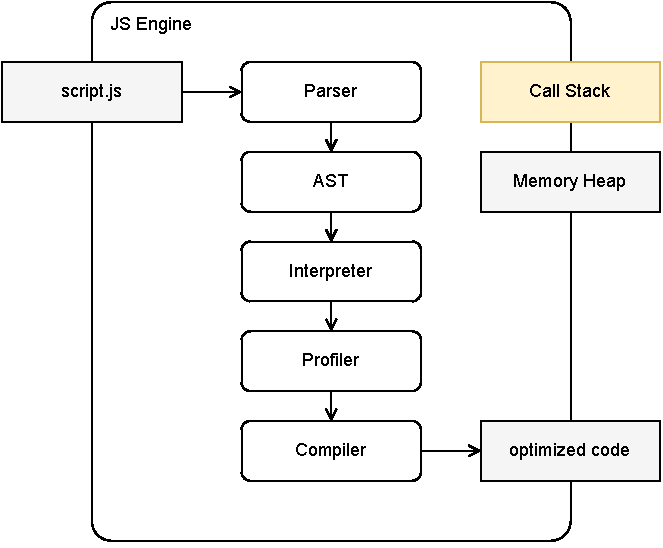
\includegraphics[width=0.5\textwidth]{includes/figures/defi_js_engine.pdf}
    \end{center}
\end{defi}

\begin{example}{Einbindung von JavaScript}
    \texttt{index.html}
    \begin{lstlisting}[language=HTML5]
        <!DOCTYPE html>
        <html>
        <head>
            <title>Index</title>
            <link rel="stylesheet" href="style.css" />
            ^<script src="script.js"></script>^
        </head>
        </html>
    \end{lstlisting}

    Die gesamte Anfrage sieht z. B. wie folgt aus\footnote{Die Datei \texttt{script.js} muss dabei statisch ausgeliefert werden}:

    \begin{center}
        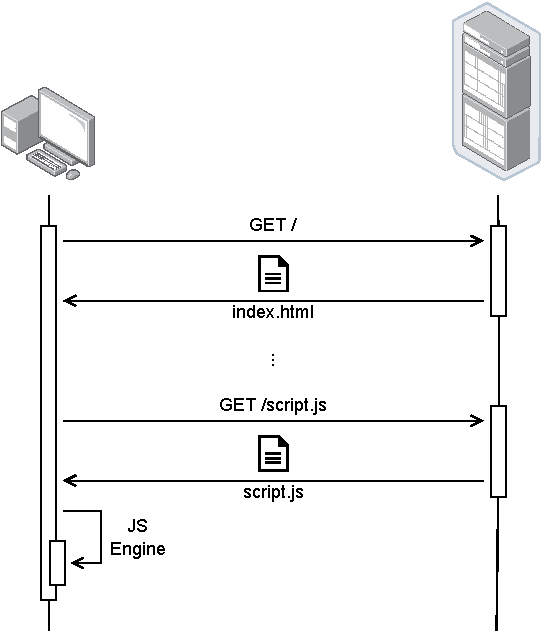
\includegraphics[width=0.50\textwidth]{includes/figures/defi_client_js.pdf}
    \end{center}
\end{example}

\begin{example}{Einbindung von JavaScript (deprecated)}
    \texttt{index\_deprecated.html}:

    \begin{lstlisting}[language=HTML5]
        <!DOCTYPE html>
        <html>
        <head>
            <title>Index</title>
        </head>

        <body>
            <button onclick="doStuff();">Klick mich!</button>
            <script>alert('Willkommen!');</script>
        </body>
        </html>
    \end{lstlisting}

    Problem: Keine Trennung von HTML und JavaScript!
\end{example}

\begin{defi}{Variablen (JavaScript)}
    \emph{Variablen} haben in JavaScript keinen festen Typen.
    Nicht initialisierte Variablen haben den Wert \texttt{undefined}.

    Zur Deklaration von Variablen stehen 3 Schlüsselworte zur Verfügung:

    \begin{tabularx}{\textwidth}{|l|X|X|}
        \hline
        Schlüsselwort & Beschreibung                                                                                                                            & Gültigkeitsbereich                                                                       \\\hline\hline
        var           &                                                                                                                                         & Innere sowie äußere Scopes innerhalb der Funktion, in der die Variable deklariert wurde. \\\hline
        let           & Vergleichbar mit dem aus \texttt{Java} bekannten Schlüsselwort \texttt{var}                                                             & Scope, in dem die Variable deklariert wurde, sowie innere Scopes                         \\\hline
        const         & Wie \texttt{let}, jedoch müssen const Variablen bei der Deklaration initialisiert werden und können danach nicht mehr angepasst werden. &                                                                                          \\\hline
    \end{tabularx}
\end{defi}

\begin{bonus}{Besonderheiten (JavaScript)}
    JavaScript arbeitet intern mit folgenden Datentypen\footnote{Primitive Datentypen werden als Kopie übergeben, Objekte als Referenz}:

    \begin{tabular}{|l|l|}
        \hline
        Typ                                   & Literal                                                     \\\hline\hline
        \texttt{boolean}                      & \texttt{true}, \texttt{false}                               \\\hline
        \texttt{number}                       & \texttt{0}, \texttt{7.5}, \texttt{1.2e5}                    \\\hline
        \texttt{string}                       & \texttt{`stringf \$\{value\}`}, \texttt{'normal string'}    \\\hline % TODO Quote
        \texttt{function}                     & \texttt{function(param) \{...\}}, \texttt{param => \{...\}} \\\hline
        \texttt{undefined}                    & \texttt{undefined}                                          \\\hline
        \texttt{object} (oberstes Kernobjekt) & \texttt{\{\}}                                               \\\hline
    \end{tabular}

    Beim Vergleichen von Variablen stehen einem zwei Operatoren zur Verfügung:
    \begin{itemize}
        \item \texttt{==}: Versucht verschiedene Datentypen sinnvoll zu vergleichen
        \item \texttt{===}: Vergleicht nur gleiche Datentypen.
              Unterschiedliche Datentypen geben immer \texttt{false} zurück.
    \end{itemize}

    \emph{Falsy Values} geben bei der Typumwandlung\footnote{explizit oder implizit z. B. in dem Kopf einer Schleife} in einen \texttt{boolean} \texttt{false} zurück.
    Zu falsy Values gehören \texttt{false}, \texttt{0}, \texttt{""}, \texttt{null}, \texttt{undefined}, \texttt{NaN}.
    Alle anderen Objekte sind \emph{truthy values}.

    \emph{Arrays} haben keine feste Größe und keinen festen Datentypen.

    Klassenattribute müssen immer mit \texttt{this.} adressiert werden.
\end{bonus}

\begin{example}{JavaScript}
    \begin{lstlisting}[language=JavaScript]
        let glumanda = {
            id: 4,             // number
            name: 'Glumanda',  // string
            typ: 'Feuer'       // string
            groesse: 0.6       // number
            attacken: [        // array
                'Glut', 'Flammenwurf', 'Drachenwut', 'Schaufler'
            ]

            to_string: () => `${this.name} [${this.id}]` // function
            attack: i => console.log(attacken[i])        // function
        }

        console.log(glumanda.id)             // 4
        console.log(glumanda.vorentwicklung) // undefined
        console.log(glumanda.to_string())    // Glumanda [4]
        glumanda.attack(2)                   // Flammenwurf
        // glumanda.attack(5)                // Error
        glumanda.attacken[5] = 'Fliegen'     // ok
        glumanda.attack(5)                   // Fliegen
    \end{lstlisting}
\end{example}

\begin{example}{JavaScript Vererbung}
    \begin{lstlisting}[language=JavaScript]
        class Pokemon {
            id, name, typ // nicht notwendig, jedoch sinnvoll

            constructor(id, name, typ) {
                this.id = id
                this.name = name
                this.typ = typ
            }

            to_string() {
                return `${this.name} [${this.id}]`
            }
        }

        class FeuerPokemon extends Pokemon {
            brennen() {
                console.log('*knister*')
            }
        }

        let glumanda = new Pokemon(4, 'Glumanda', 'Feuer')
        console.log(glumanda.to_string()) // Glumanda [4]
        // glumanda.brennen               // undefined

        let glutexo = new FeuerPokemon(5, 'Glutexo', 'Feuer')
        console.log(glutexo.to_string()) // Glutexo [5]
        // glutexo.brennen               // function
        glutexo.brennen()                // *knister*
    \end{lstlisting}
\end{example}

\begin{bonus}{Klassenlose Vererbung (JavaScript)}
    Jede Instanz einer Klasse hat ein verstecktes Attribut \texttt{\_\_proto\_\_}.

    Jede Klasse hat ein verstecktes Attribut \texttt{prototype}.

    Wenn man auf ein Attribut eines Objektes zugreifen möchte, welches dort nicht direkt gefunden wird, schaut die Engine in dem jeweiligen Prototypen nach.
    Sollte es dort nicht gefunden werden, wird rekursiv eine Ebene höher geschaut.
\end{bonus}

\begin{example}{Klassenlose Vererbung (JavaScript)}
    \begin{lstlisting}[language=JavaScript]
        let glumanda = {
            id: 4
            name: 'Glumanda'
        }
        glumanda.__proto__.typ = 'Feuer'
        glumanda.__proto__.name = 'Philipp'

        console.log(glumanda.name)           // Glumanda
        console.log(glumanda.__proto__.name) // Philipp
        console.log(glumanda.typ)            // Feuer (aus __proto__)
        console.log(glumanda.brennen)        // undefined
    \end{lstlisting}
\end{example}

\begin{defi}{Call Stack (JavaScript)}
    Der \emph{Call Stack} führt Methoden synchron aus.

    Die Reihenfolge wird nach dem LIFO Prinzip entschieden.

    Ob Methoden in den \emph{Call Stack} aufgenommen werden, wird durch den \emph{Event Loop} entschieden
\end{defi}

\begin{defi}{Callback Queue (JavaScript)}
    Wenn WEB APIs JavaScript Code ausführen müssen, werden die Methoden in die \emph{Callback Queue} eingefügt.

    Die Reihenfolge wird nach dem FIFO Prinzip entschieden.

    Wenn der \emph{Call Stack} leer ist, wird das älteste Objekt der \emph{Callback Queue} dorthin verschoben.
\end{defi}

\begin{defi}{JavaScript Runtime Environment}
    JavaScript blockiert dem Main Thread nicht.
    Alle Funktionen werden aus dem Source Code direkt in den \emph{Call Stack} aufgenommen und ausgeführt.

    Deswegen nennt man JavaScript \emph{Single-Threaded and Non-Blocking}.

    \begin{center}
        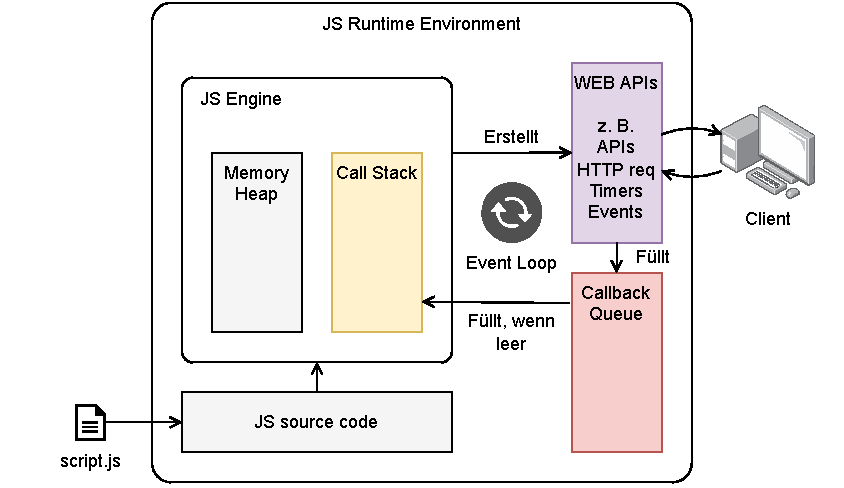
\includegraphics[width=0.75\textwidth]{includes/figures/defi_js_runtime_environment.pdf}
    \end{center}
\end{defi}

\begin{example}{Single-Threaded and Non-Blocking (JavaScript)}
    \begin{lstlisting}[language=JavaScript]
        function a() {
            console.log('a')            
        }

        a()
    \end{lstlisting}

    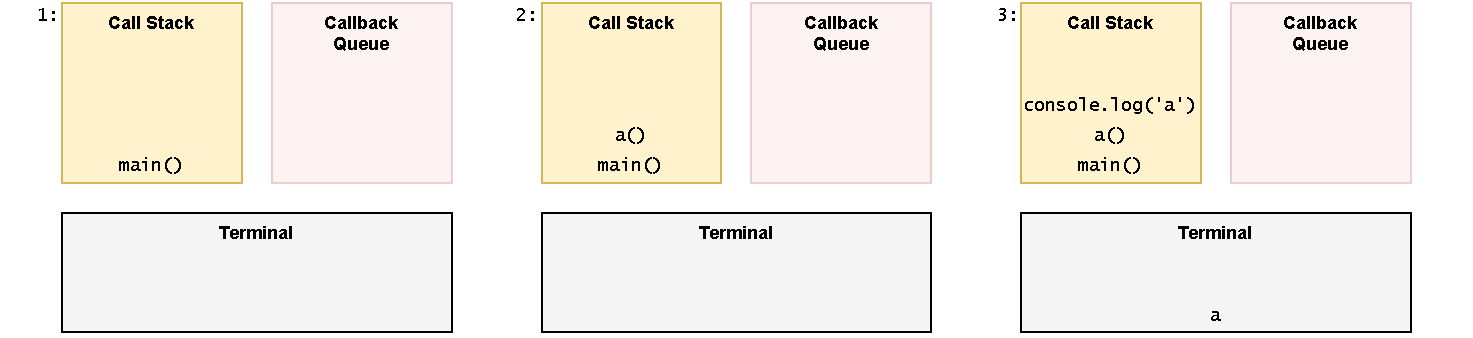
\includegraphics[width=\textwidth]{includes/figures/example_stanb_1.pdf}

    \begin{enumerate}
        \item \texttt{main()} \emph{(Call Stack)}
        \item \texttt{a()} wird in den \emph{Call Stack} eingefügt.
        \item \texttt{console.log('a')} \emph{(Call Stack)}
        \item Alle Methoden im \emph{Call Stack} werden entfernt
    \end{enumerate}
\end{example}

\begin{example}{Single-Threaded and Non-Blocking (JavaScript)}
    \begin{lstlisting}[language=JavaScript]
        setTimeout(() => {
            console.log('a')
        }, 10)

        console.log('b')
    \end{lstlisting}

    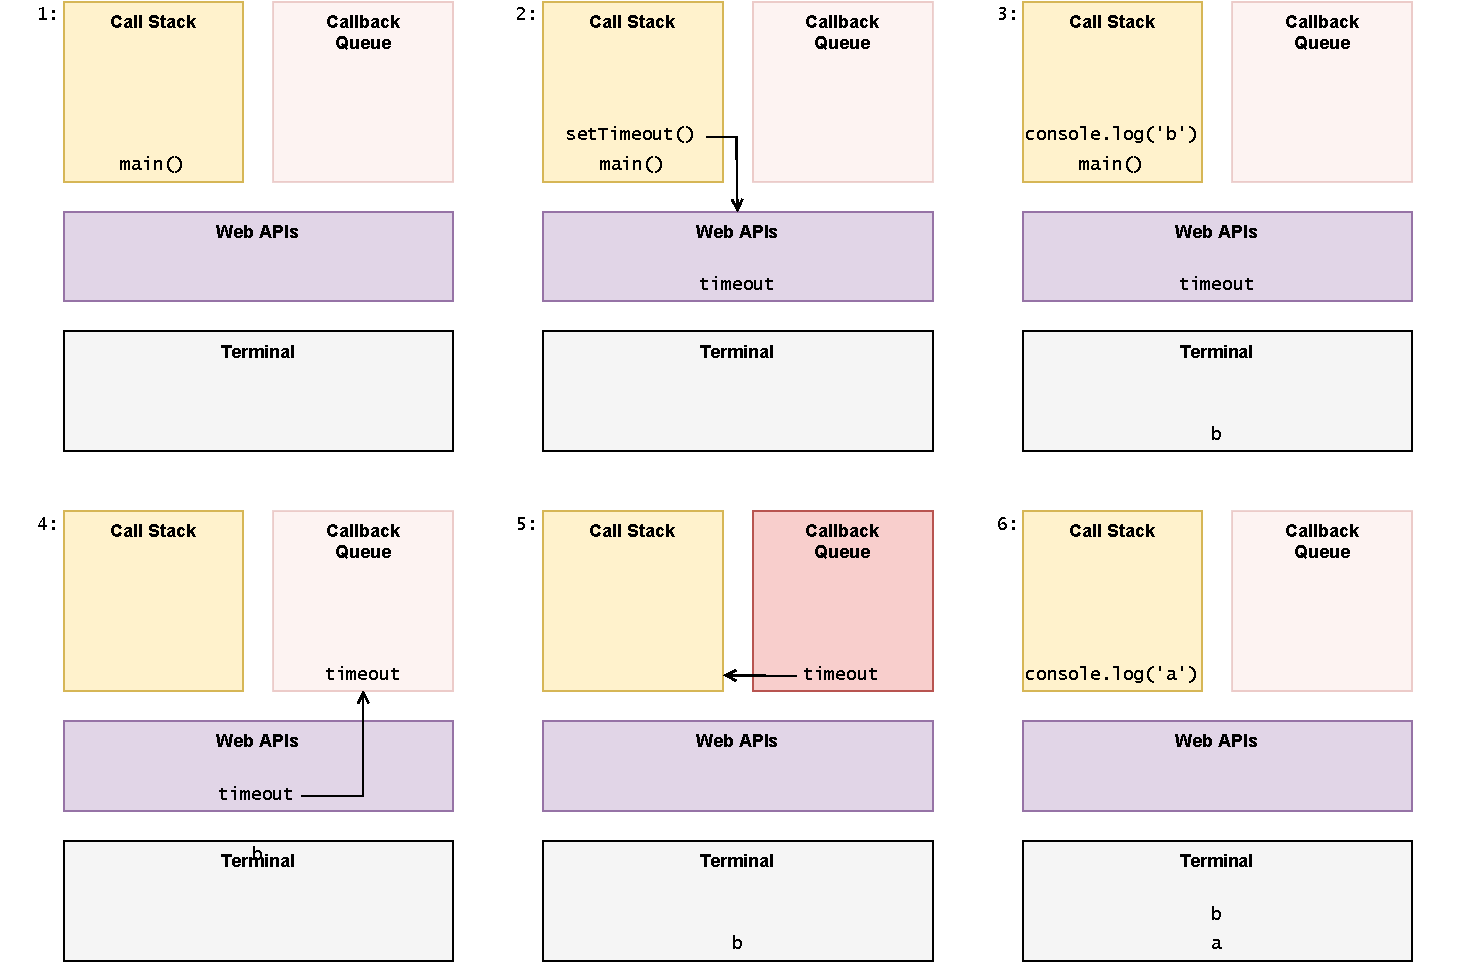
\includegraphics[width=\textwidth]{includes/figures/example_stanb_2.pdf}

    \begin{enumerate}
        \item \texttt{main()} \emph{(Call Stack)}
        \item \texttt{setTimeout()} fügt den Timer zu den \emph{Web APIs} hinzu.
        \item \texttt{console.log('b')} \emph{(Call Stack)}
        \item Nach Ablauf des Timers\footnote{Auch wenn der Timer 0 Sekunden dauert, durchläuft der Timer die gesamten Schritte, 'a' wird also nach 'b' ausgegeben} wird das interne Lambda in die \emph{Callback Queue} hinzugefügt.
        \item Da der \emph{Call Stack} leer ist, wird das Lambda direkt in den \emph{Call Stack} eingefügt.
        \item \texttt{console.log('a')} \emph{(Call Stack)}
    \end{enumerate}
\end{example}

\begin{example}{Single-Threaded and Non-Blocking (JavaScript)}
    \begin{lstlisting}[language=JavaScript]
        document.getElementById('btn').addEventListener('click', event => {
            console.log('click!')
        })

        console.log('block')
    \end{lstlisting}

    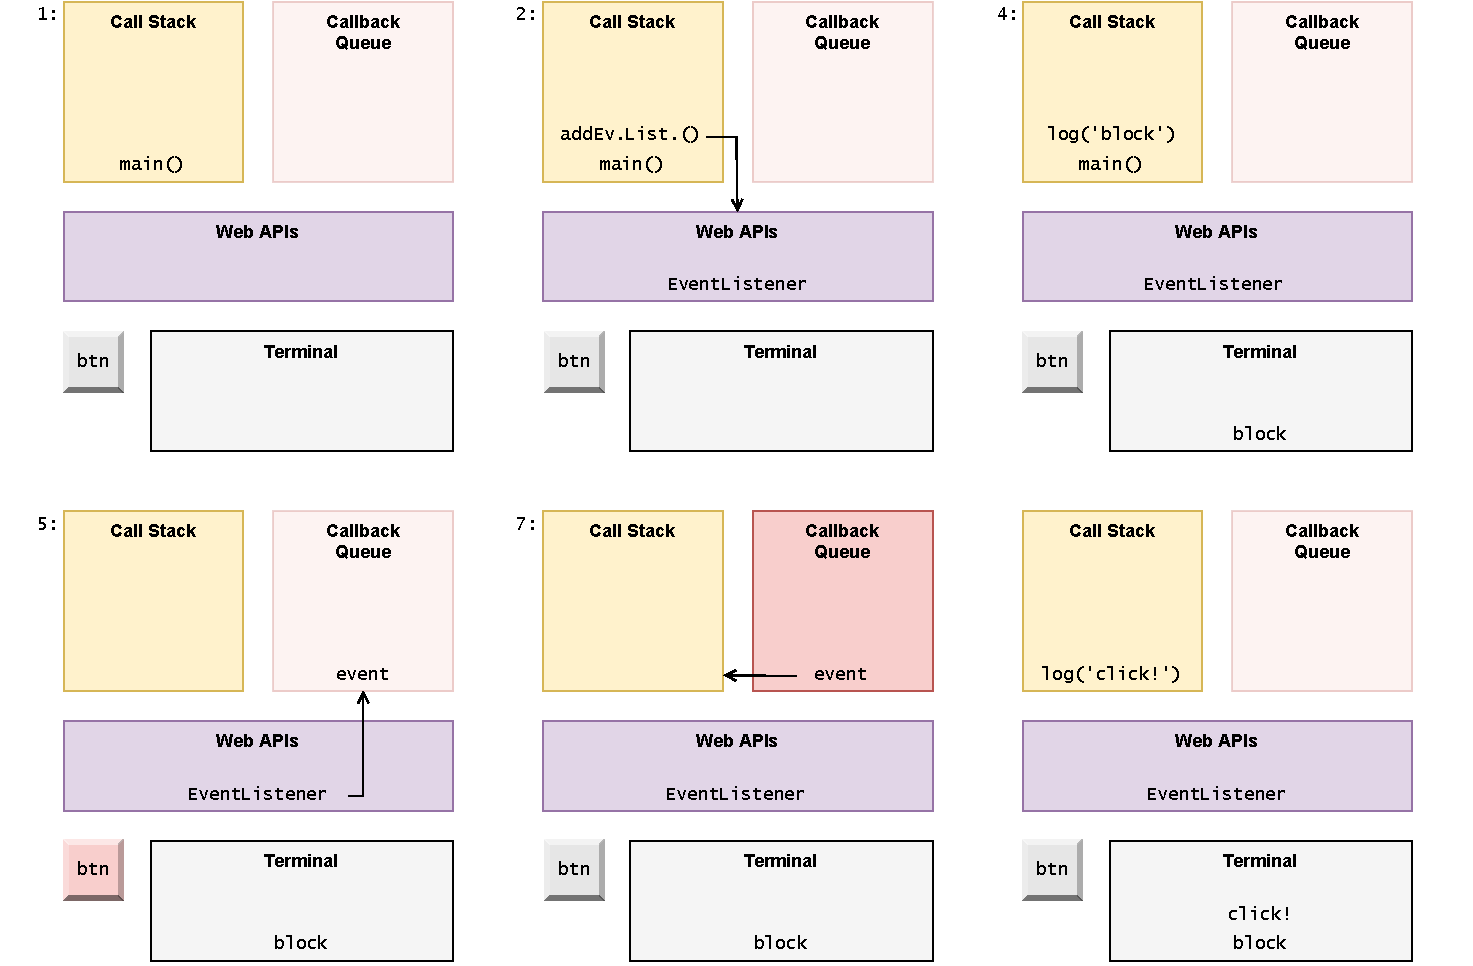
\includegraphics[width=\textwidth]{includes/figures/example_stanb_3.pdf}

    \begin{enumerate}
        \item \texttt{main()} \emph{(Call Stack)}
        \item Dem HTMLElement mit der ID \texttt{btn} wird ein \texttt{EventListener} hinzugefügt \emph{(Call Stack)}.
        \item In den \emph{Web APIs} befindet sich nun ein \texttt{EventListener}.
        \item \texttt{console.log('block')} \emph{(Call Stack)}
        \item Wenn nun irgendwann der Button gedrückt wird, fügt die \emph{Web API} ein \texttt{Event} der \emph{Callback Queue} hinzu.
        \item Wenn 3. erfolgreich ausgeführt wurde, ist der \emph{Call Stack} leer.
        \item Wenn der \emph{Call Stack} leer ist, wird \texttt{console.log('click!')} ausgeführt \emph{(Call Stack)}
        \item Ansonsten warten alle Elemente der \emph{Callback Queue} darauf, dass der \emph{Event Loop} sie \enquote{abholt}
    \end{enumerate}
\end{example}

\begin{defi}{Callbacks (JavaScript)}
    Wenn man nun trotzdem auf die Rückgabe von Funktionen warten möchte, die eine längere Laufzeit benötigen, als der Event Loop ihnen zur Verfügung stellt, muss man auf asynchrone Methoden zurückgreifen.

    Ein erster Ansatz dazu waren \emph{Callbacks}.

    Die Idee hinter Callbacks ist, dass man Methoden eine weitere Methode mitgibt, welche nach Ablauf der eigentlichen Methode mit der Rückgabe dieser als Parameter, die mitgegebene Methode ausführt.
    Callbacks haben den großen Vorteil, dass man sich die Methoden modular aufbauen kann.
    Bisher kann man nicht die tiefere Methode zur Laufzeit austauschen.
\end{defi}

\begin{example}{Callbacks (JavaScript)}
    Die folgenden Methoden erstellen einen Timer und rufen dann die Callback-Methode mit dem \enquote{passenden} Buchstaben auf.

    Die bisherige Implementierung sieht wie folgt aus:
    \begin{lstlisting}[language=JavaScript]
        function a(s) {
            /* sleep */
            b(s + 'a')
        }

        ...

        function c(s) {
            /* sleep */
            console.log(s + 'c')
        }
    \end{lstlisting}

    \begin{lstlisting}[language=JavaScript]
        a('') // abc
    \end{lstlisting}

    Die Callback-Implementierung sähe z. B. wie folgt aus:
    \begin{lstlisting}[language=JavaScript]
        function a(s, callback) {
            /* sleep */
            callback(s + 'a')
        }

        ...
    \end{lstlisting}

    \begin{lstlisting}[language=JavaScript]
        a('',
            s => b(s,
                s => c(s, 
                    console.log // abc
                )
            )
        )
    \end{lstlisting}

    Die untere Variante ist zwar modularer und offen für Erweiterungen, jedoch nicht sonderlich lesbar.
    Einen potentiellen Ausweg aus dieser Callback-Hell bietet das Promise-Interface.
\end{example}

\begin{defi}{Promise (JavaScript)}
    Ein Promise ist ein Platzhalter für eine Variable.
    Es gibt drei interne Zustände:

    \begin{center}
        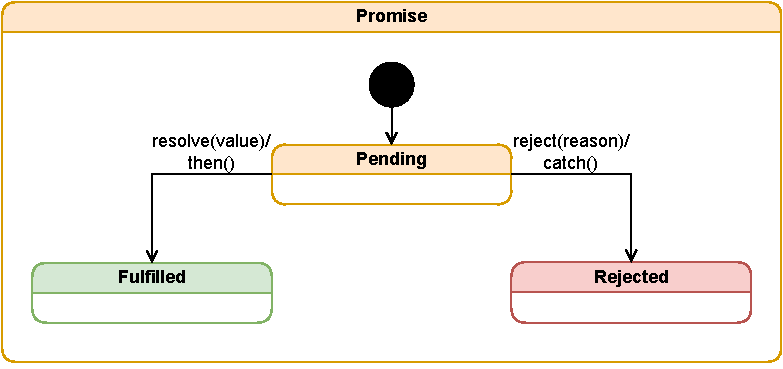
\includegraphics[width=0.5\textwidth]{includes/figures/defi_promise.pdf}
    \end{center}

    Bei der Erstellung eines Promises übergibt man zwei Callbacks\footnote{Diese werden den \emph{Web APIs} hinzugefügt}:
    \begin{lstlisting}[language=JavaScript]
        const p = new Promise((resolve, reject) => { ... })
    \end{lstlisting}

    Wenn der Promise in \texttt{Fulfilled} wechselt, kann man direkt eine weitere \texttt{then()} Methode mit dem \texttt{value} aufrufen.
    \texttt{then()} erstellt im Hintergrund einen weiteren Promise.

    Wenn der Promise in \texttt{Rejected} wechselt, springt der Promise in die \texttt{catch()} Methode.

    Zum Schluss kann man eine \texttt{finally()} Methode ausführen lassen.
\end{defi}

\begin{example}{Promise (JavaScript)}
    Um auf unser Beispiel zurück zu kommen:
    \begin{lstlisting}[language=JavaScript]
        function a(s) {
            return new Promise((resolve, reject) => {
                /* sleep */
                resolve(s + 'a')
            })
        }
    \end{lstlisting}

    \begin{lstlisting}[language=JavaScript]
        a('')
            .then(s => b(s))
            .then(s => c(s))
            .then(console.log) // abc
    \end{lstlisting}
\end{example}

\begin{example}{Promise Error (JavaScript)}
    Sollte \texttt{b} einen Fehler werfen, können wir diesen Fehler am Ende der \texttt{then()}-Kette mit \texttt{catch()} abfangen.
    Ab der Methode, in der der Fehler geworfen wird, werden nur noch \texttt{catch()} sowie \texttt{finally()} beachtet.

    % TODO .then() weniger Deckkraft
    \begin{lstlisting}[language=JavaScript]
        a('')
            ^.then(s => b(s))^                     // error
            .then(s => c(s))                     // skip
            .then(console.log)                   // skip
            ^.catch(err => console.log('Fehler'))^ // Fehler
    \end{lstlisting}
\end{example}

\begin{defi}{Asynchronität (JavaScript)}
    Da, je nach Komplexität, auch \texttt{.then()}-Ketten unübersichtlich werden.
    Um dort Abhilfe zu schaffen, wurden \texttt{async}-Methoden hinzugefügt.
    In dieser Methode kann man mit \texttt{await} darauf warten, dass ein Promise in den Fulfilled Zustand wechseln.
\end{defi}

\begin{example}{Asynchronität (JavaScript)}
    \begin{lstlisting}[language=JavaScript]
        function a(s) {
            return new Promise((resolve, reject) => {
                /* sleep */
                resolve(s + 'a')
            })
        }
    \end{lstlisting}

    \begin{lstlisting}[language=JavaScript]
        ^async^ function abc() {
            // console.log(a(''))       // Promise
            // console.log(await a('')) // a
            let s = ''
            s = ^await^ a('')
            s = ^await^ b(s)
            s = ^await^ c(s)
            console.log(s) // abc
        }
        abc()
    \end{lstlisting}
\end{example}

\begin{bonus}{Asynchronität mehrerer unabhängiger Promises (JavaScript)}
    Asynchrone Methoden sollten trotzdem möglichst schnell sein.
    Wenn verschiedene Promises unabhängig sind, sollten diese nicht aufeinander warten müssen.

    \begin{lstlisting}[language=JavaScript]
        async function abc() {
            const s1 = await a('')
            const s2 = await b('')
            const s3 = await c('')

            console.log(s1 + s2 + s3) // abc
        }
        abc()
    \end{lstlisting}
    In diesem Beispiel ist nur \texttt{console.log} abhängig von den vorherigen Methoden.
    Trotzdem muss \texttt{b()} auf \texttt{a()} warten.

    Besser und schneller\footnote{
        Die Methoden geschehen nicht gleichzeitig, da JavaScript ausschließlich auf einem Thread läuft.
        Jedoch stückelt die Engine die Methoden in kleinere Stücke, die abwechselnd ausgeführt werden.
    } ist:
    \begin{lstlisting}[language=JavaScript]
        async function abc() {
            const [s1, s2, s3] = await Promise.all([
                a(''), b(''), c('')
            ])

            console.log(s1 + s2 + s3) // abc
        }
        abc()
    \end{lstlisting}
\end{bonus}

\subsection{Fetch}

\begin{defi}{DOM}
    Eine HTML Webseite ist als Baumstruktur im \emph{Document Object Model (DOM)}-Format gespeichert.

    Die Wurzel stellt dabei immer das \texttt{HTML}-Objekt dar.
    In JavaScript kann man durch den Baum navigieren und die Objekte manipulieren.
\end{defi}

\begin{defi}{DOM-Manipulation (JavaScript)}
    Zur Manipulation von DOM-Objekten stehen zwei globale Variablen zur Verfügung:
    \begin{itemize}
        \item \texttt{document}: Die geladene Webseite.
              Die Variable \texttt{document} ist eine Instanz des Interfaces \texttt{Document} und dient als Einstiegspunkt in den Inhalt der Webseite.

              Einige der relevanten Methoden des Objektes sind:
              \begin{itemize}
                  \item \texttt{getElementById()}: Gibt ein bestimmtes \texttt{HTMLElement} zurück.
                  \item \texttt{getElementByClassName()}: Gibt eine HTMLCollection aller \texttt{HTMLElemente} zurück, die diese Klasse in ihrer \texttt{classList} haben.
              \end{itemize}
        \item \texttt{window}: Eine Repräsentation des geladenen Fensters.

              Die Variable wird genutzt um auf den fertigen Aufbau von dem \texttt{document} zu warten oder die Seite umzuleiten.
    \end{itemize}

    Des Weiteren benötigen wir einige mitgelieferten Klassen:
    \begin{itemize}
        \item \texttt{HTMLElement}: Ein spezifisches Element.

              Einige relevante Member der Klasse sind:
              \begin{itemize}
                  \item \texttt{textContent}: z. B. der Text eines Buttons
                  \item \texttt{value}: z. B. die Eingabe einer Textbox
                  \item \texttt{disabled}: Boolean um Eingabeobjekte zu deaktivieren
                  \item \texttt{classList}: Liste aller Klassen
                  \item \texttt{addEventListener()}: Zum Hinzufügen eines \texttt{EventListeners}
              \end{itemize}
        \item \texttt{HTMLCollection}: Eine Array-ähnliche Sammlung an \texttt{HTMLElementen}

              Neben ein paar Membern (wie z. B. \texttt{length}) bieten HTMLCollections keine Funktionen.
              Wenn man über alle HTMLElemente einer HTMLCollection iterieren möchte, muss man sich aus der Collection ein Array erstellen:

              \texttt{Array.from(HTMLCollection).foreach(element => {...})}
        \item \texttt{Event}: Ein Event wird durch spezifische Nutzungseingaben ausgelöst.

              Einige relevante Member der Klasse sind:
              \begin{itemize}
                  \item \texttt{target}: Das auslösende HTMLElement
                  \item \texttt{preventDefault()}: Bricht das Event ab (z. B. wenn man die Aktion einer Form nicht auslösen möchte)
              \end{itemize}
    \end{itemize}
\end{defi}

\begin{example}{DOM-Manipulation (JavaScript)}
    \begin{lstlisting}[language=JavaScript]
        window.onload = () => {
            ...
        }

        let btn = document.getElementById('...') // HTMLElement
        btn.addEventListener('click', event => {
            ...
        })

        Array
            .from(
                document.getElementByClassName('...') // HTMLCollection
            )
            .foreach(element => ...)
    \end{lstlisting}
\end{example}

\begin{bonus}{Ajax}
    Neben einfacher DOM-Manipulation bietet JavaScript einem die Möglichkeit in den clientseitig ausgeführten Skripten mit dem Server zu kommunizieren.
    Der Datenaustausch findet dabei in XML oder JSON statt.

    Die erhaltenen Daten werden dann clientseitig in das DOM Dokument eingebunden.

    Vorteile:
    \begin{itemize}
        \item Verringerte Serverlast
        \item Erhöhte Benutzungsfreundlichkeit
    \end{itemize}

    Nachteile
    \begin{itemize}
        \item Bruch mit klassischen Technologien
        \item Komplexität der URL-Ressource hoch
        \item Suchmaschinenlesbarkeit erschwert
    \end{itemize}
\end{bonus}

\begin{example}{Ajax (Deprecated)}
    \begin{lstlisting}[language=JavaScript]
        const xmlHttp = new XMLHttpRequest()

        xml.onreadystatechange = () => {
            if (xml.readyState = XMLRequest.DONE)
                console.log(xmlHttp.responseText)
        }

        xmlHttp.open('GET', 'http://paddel.xyz', true)
        xmlHttp.send(null)
    \end{lstlisting}

    xmlHttp funktioniert zwar, jedoch gelingt man schnell in eine Callback-Hell und ist gezwungen mit XML arbeiten.

    Moderne Schnittstellen arbeiten mit \texttt{fetch}.
    \texttt{fetch} arbeitet mit Promises und gibt JSON Objekte zurück.
\end{example}

\begin{example}{Ajax}
    \begin{lstlisting}[language=JavaScript]
        fetch(url)
            .then(res => res.json()) // parsed Erhaltene response in Json
            .then(data => {
                ...
            })
            .catch(err => {
                ...
            })
    \end{lstlisting}
\end{example}

\begin{example}{Ajax (GET)}
    \begin{lstlisting}[language=JavaScript]
        fetch('https://paddel.xyz/pokemon?id=4')
            .then(res => res.json())
            .then(console.log) // Glumanda [4]
    \end{lstlisting}
\end{example}

\begin{example}{Ajax (POST)}
    \begin{lstlisting}[language=JavaScript]
        fetch('https://paddel.xyz/pokemon',
            {
                'method': 'POST',
                'body': { 'id': 4 },
                'headers': { 'Content-Type': 'application/json' }
            }
        )
            .then(res => res.json())
            .then(console.log) // Glumanda [4]
    \end{lstlisting}
\end{example}